\chapter{Interoperability of clouds}

\chapterintro{This chapter introduces the notion of a hybrid cloud and explains its role in IT industry. On top of this deployment model, the concept of InterCloud is presented and elaborated with the emphasis on its application in ensuring scalability of users' services.}

\section{Introduction}
From the perspective of a user of PaaS services it is vital that they are able to deploy seamlessly their applications using libraries, tools and services supported by the cloud provider\cite{MeGr11}. Judging by such factors as the popularity of Heroku -- currently one of the most popular PaaS providers which does not offer more advanced features which would enable management of the infrastructure underpinning the deployment platform, the fact that Microsoft added auto-scaling to its Azure platform as late as in June 2013, it is perfectly possible most PaaS users are satisfied with the current offers of their providers and do need another, more sophisticated functionalities. However, there are more complex applications and systems whose requirements regarding technology stack, availability and scalability are considerably more demanding. For such services there ought to be designed slightly specialized features that would require cooperation among different cloud providers.

\section{Hybrid cloud}
One can imagine scenarios in which customers of cloud services know their applications are vulnerable to sudden variations in demand and their responsiveness must be kept at the same level all the time. In such cases, they want them to scale dynamically according to current load or other predefined or manually specified metrics. What is more, in order to ensure high availability of their services, customers do not want to confine themselves to only one provider -- in the best scenario they want their applications (or their logical parts, such as persistence layer) to be spanned across different providers and be able to cooperate with one another at the same time. Additionally, due to privacy concerns of the sensible data, companies are reluctant to put it in the public cloud storage. All these factors lead to the concept of a \emph{hybrid cloud}\cite{MeGr11} -- the case in which the cloud is a composition of two or more distinct infrastructures which are unique entities, but there are technological means that make it possible to port data and applications among them.

\subsection{Deployment models}
The informal introduction to the concept of a \emph{hybrid cloud} in the previous section requires a strict definition, but it is virtually impossible without defining other deployment models:
\begin{itemize}
  \item Private Cloud -- The provisioned cloud infrastructure is used exclusively by a single organization (that may consist of many business units) and may be owned, managed and operated by the organization or a third party.
  \item Public Cloud -- The provisioned cloud infrastructure is used by general public and may be owned, managed and operated by a business, academic or government organization or some combination of them. It exists on the premises of the cloud provider.
  \item Community Cloud -- The cloud infrastructure is provisioned for exclusive use by a specific community of consumers from organizations that have shared concerns (e.g., mission, security requirements, policy , and compliance considerations). It may be owned, managed , and operated by one or more of the organizations in the community, a third party, or some combination of them, and it may exist on or off premises. 
\end{itemize}
Having defined those models, we can see that \emph{hybrid cloud} can be placed among them and be defined as a model in which the provisioned infrastructure is a composition of two or more other infrastructures - \emph{private},\emph{community} or \emph{public}.

\subsection{Current usage and trends}
\subsubsection*{Cloud -- clients' view}
Before digging into the details of current usage and popularity of the hybrid model, it is worth discussing the general attitude of clients towards cloud computing. As the recent survey \cite{NBSurvey13} shows, the major factor that prevents companies from adopting cloud solutions is their concern over security -- in 2012 as much as 52\% responders considered it as a main concern with the regard to cloud in general. However, the tendency is that more and more enterprises do not find it a major issue as in 2012 the number declined to 46\%.
Complexity related to the management of cloud components, Vendor lock-in, interoperability and reliability were among the most frequent obstacles to adoption in 2013 for they constituted 46\%, 35\%, 27\% and 22.3\% of responders' votes respectively. Total results are shown in the figure \ref{ch4:cloud-computing-adoption-obstacles-2013}.
\begin{figure}[!ht]
  \begin{center}
    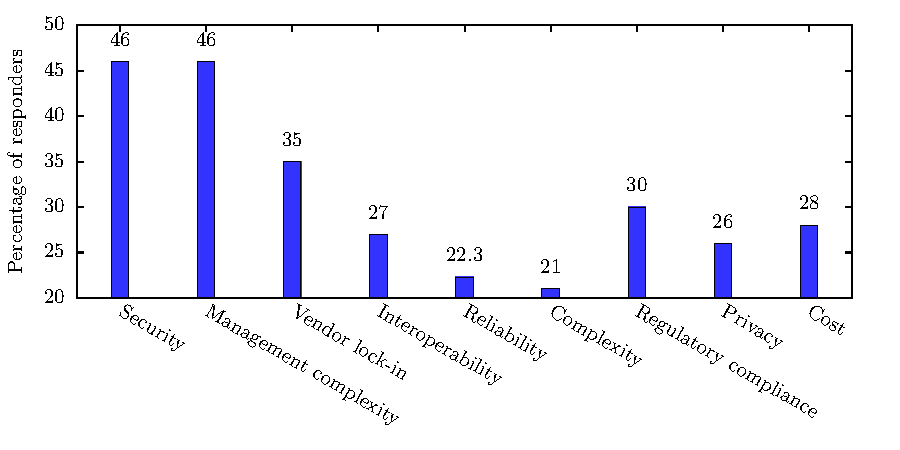
\includegraphics{chapter-4/cloud-computing-adoption-obstacles-2013}
  \end{center}
  \caption{Major obstacles to cloud adoption in 2013 according to \cite{NBSurvey13}}
  \label{ch4:cloud-computing-adoption-obstacles-2013}
\end{figure}

The same survey shows that the cloud adoption growth rate is high -- 75 percent of responders stated usage of some sort of a cloud platform. This means 8 percent growth when compared to the results obtained in 2012. The expectations for the total worldwide addressable market for cloud computing are to reach \$158.8B by 2014 -- an increase of 126.5 percent from 2011.

\subsubsection*{View on hybrid cloud}
When it comes to the application of a hybrid model in industry, in most cases the definition introduced in the previous chapter now becomes a 'public-private' composition. And this is how the term should be understood when discussing the results of the surveys which aimed to provide insights onto the view on a hybrid cloud from the customers' perspective.
The study \cite{NBSurvey13} forecasts 16 percentage growth in the hybrid cloud adoption in 5 years, from 27 to 43 percent. At the same time, the usage of a public model will decline from 39 to 32 percent.
The other survey, conducted by Rackspace \cite{RackspaceSurvey13}, provides more detailed data about current usage and popularity of a hybrid model. The first interesting finding is that as much as 60\% responders, which included 1300 companies in the UK and US, have moved or are planning to move certain applications either partially (41\%) or completely (19\%) off the public cloud because of its limitations or the potential benefits of other models, e.g. the hybrid one. The second one is about the pros of adopting the hybrid cloud  -- potential users find more control (59\%) and better security (54\%) top benefits of using this deployment model. The other most responded benefits are shown in the figure \ref{ch4:hybrid-cloud-top-benefits}.

\begin{figure}[!ht]
  \begin{center}
    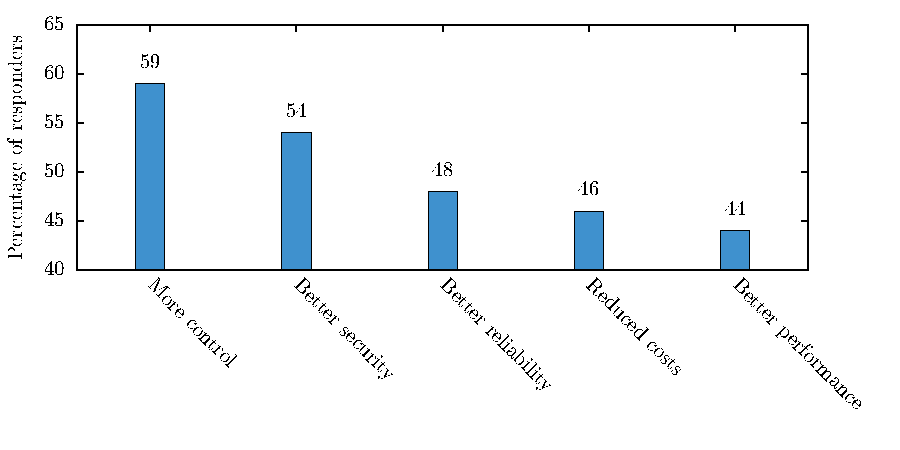
\includegraphics{chapter-4/hybrid-cloud-top-benefits}
  \end{center}
  \caption{Top benefits of using the hybrid model according to \cite{RackspaceSurvey13}}
  \label{ch4:hybrid-cloud-top-benefits}
\end{figure}

\section{Federation of clouds -- InterCloud}
As stated in the previous sections, one of the major obstacles that prevents consumers from adopting cloud solutions is reliability. It appears that these statements are not only imaginary worries of entrepreneurs, but real problems -- there are cases, where some providers temporarily run short of capacity (e.g. because of provisioning too many virtual machines) in the face of hight demand \cite{Lavitt09}. What is more, the more demanding clients require specific QoS to be satisfied by their providers as negotiated in Service Level Agreements.
In order to meet these challenges there is a need of a completely new approach to the problem of effective management of resources. The new solution should take into account such factors as:

\begin{itemize}
  \item users' requests priority
  \item users' QoS requirements (e.g. the deadline by which some jobs have to be executed)
  \item price that the clients pay for the usage of resources
\end{itemize}

Computer scientists in the field of cloud computing devised a model \cite{MarketOrientedCC08} in which resources are managed in a market-oriented fashion that enables dynamic regulation of the supply and demand of resources and promotes the mechanisms for their allocation that would take into account their priorities and levels of utilization.
The extension of this model is a vision of creating the federated cloud computing environment, so called \emph{InterCloud}, that ``facilitates just-in-time, opportunistic, and scalable provisioning of application services, consistently achieving QoS targets under variable workload, resource and network conditions'' \cite{InterCloud10}.
The elements of the proposed architecture are as follows:
\begin{itemize}
  \item Cloud Exchange -- acts as a market maker for bringing together both producers and consumers of services. It allows Cloud Brokers and Cloud Coordinators to match consumers with the fitting offers from providers. Such a market is a step forward towards creating a dynamic infrastructure for trading based on Service Level Agreements.
  \item Cloud Coordinator -- manages the instance of a cloud and its membership in the overall federation; provides an environment (programming, deployment) for applications
  \item Cloud Broker -- acts on behalf of the client; communicates with the Cloud Exchange to find the best cloud instances for the application
\end{itemize}

\subsection{Usage in industry}
The depicted model has not yet been adopted in the industry, yet some simulations were carried out on a \emph{CloudSim} platform and the obtained results showed that this concept has ``immense potential'' \cite{InterCloud10}.

